%%% template.tex
%%%
%%% This LaTeX source document can be used as the basis for your technical
%%% paper or abstract. Intentionally stripped of annotation, the parameters
%%% and commands should be adjusted for your particular paper - title, 
%%% author, article DOI, etc.
%%% The accompanying ``template.annotated.tex'' provides copious annotation
%%% for the commands and parameters found in the source document. (The code
%%% is identical in ``template.tex'' and ``template.annotated.tex.'')

\documentclass[conference]{acmsiggraph}

\usepackage{authblk}
\usepackage[]{algorithm2e}

\TOGonlineid{45678}
\TOGvolume{0}
\TOGnumber{0}
\TOGarticleDOI{1111111.2222222}
\TOGprojectURL{}
\TOGvideoURL{}
\TOGdataURL{}
\TOGcodeURL{}

\title{Performance Driven Redundancy Optimization of Data Layouts for Walkthrough Applications}

%\author[1]{Zachary DeStefano\thanks{zdestefa@uci.edu}}
%\author[1]{Shan Jiang\thanks{sjiang1714@gmail.com}}
%\author[1]{Gopi Meenakshisundaram\thanks{gopi.meenakshisundaram@gmail.com}}
%\author[2]{Sung-Eui Yoon\thanks{toinsert}}
%\pdfauthor{Zachary DeStefano,Shan Jiang,Gopi Meenakshisundaram,Sung-Eui Yoon}
\pdfauthor{}
\author{}
%\affil[1]{University of California, Irvine}
%\affil[2]{KAIST}

\keywords{Data Layout Problem, Out-Of-Core Rendering, Cache Oblivious Mesh Layout, Redundant Data Layout, Walkthrough Application}

\begin{document}

%% \teaser{
%%   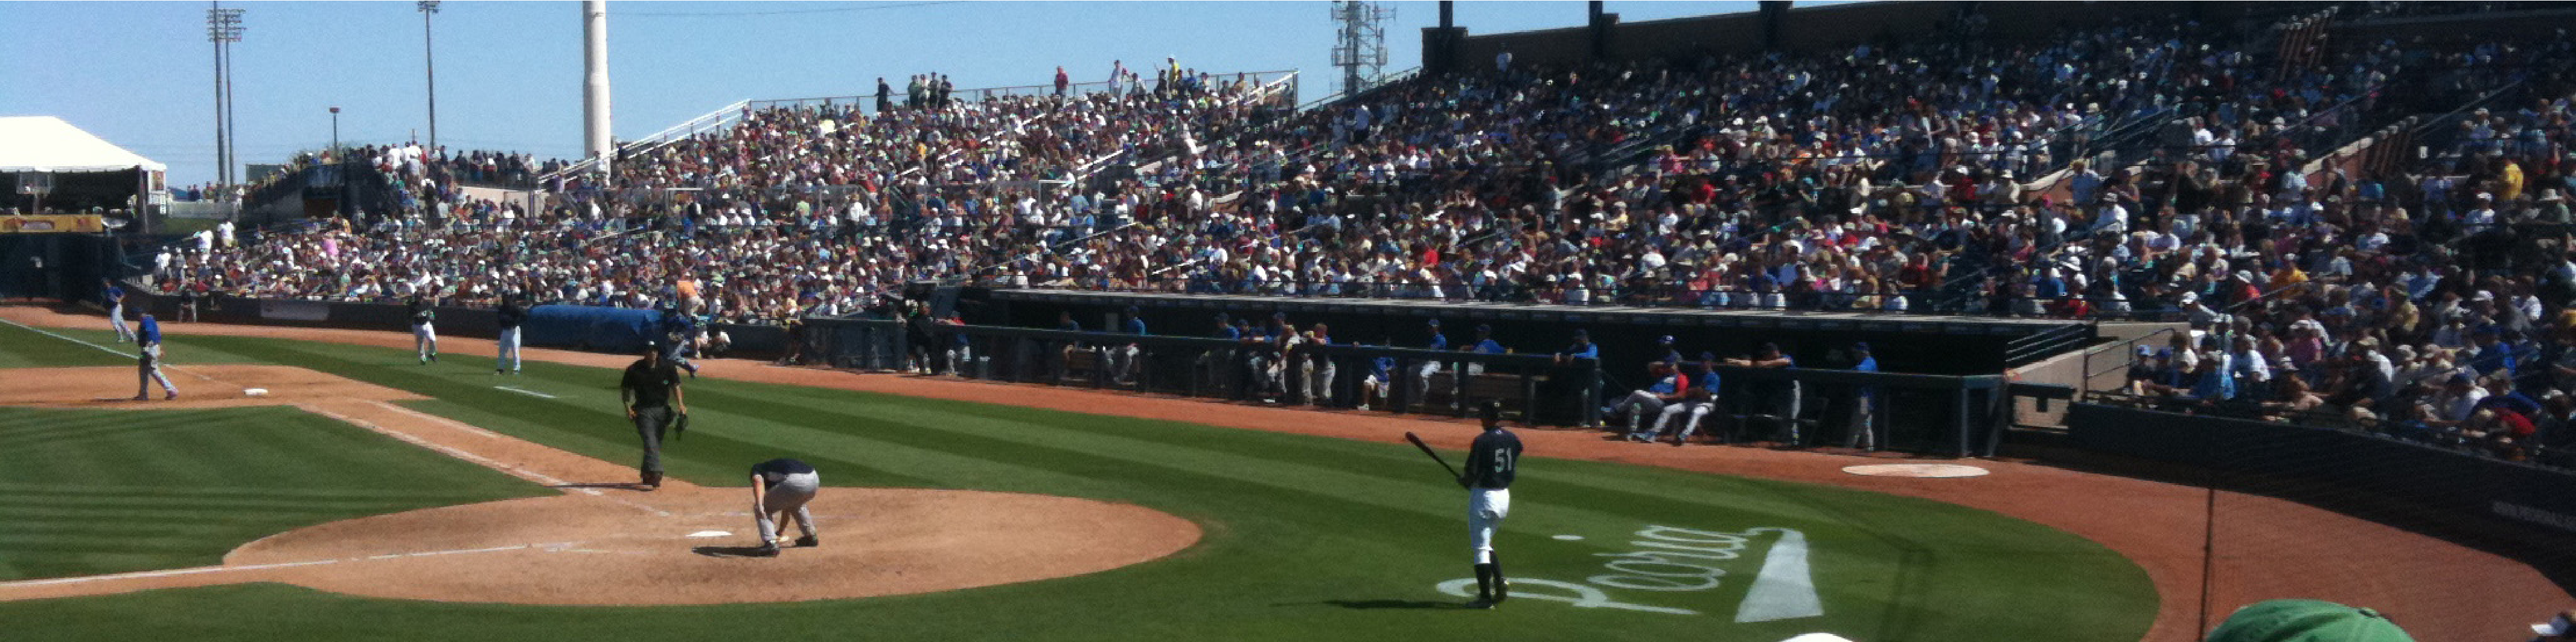
\includegraphics[height=1.5in]{images/sampleteaser}
%%   \caption{Spring Training 2009, Peoria, AZ.}
%% }

\maketitle

\section{Related Work}

Massive model rendering is a well studied problem in computer graphics. Most of the early works focused on increasing the rendering efficiency. At that time the fundamental problem was not fitting the model into the main memory but the speed of the graphics cards. Hence these works provided solutions to reduce the number of primitives to be rendered while maintaining the visual fidelity. These solutions included level-of-detail for geometric models \cite{Luebke02}, progressive level of detail \cite{Hoppe:98b,Hoppe:97,Hoppe:96,SG:01}, and image based simplification \cite{Aliaga,Hansong,Zhang}. Soon thereafter the size of the main memory became the bottleneck in handling ever increasing sizes of the model. Hence memory-less simplification techniques \cite{Lindstrom}  and other out-of-core rendering systems \cite{Correa,Varadhan} emerged in which just the limited amount of required data that needs to be processed and rendered was brought from the secondary storage to the main memory. \\
\\
Soon afterward, the researchers realized that the speed at which this data could be brought from the secondary to the main memory in these out-of-core algorithms is limited by the data bus speed, disk seek time, and data transfer time. They realized that these issues could be ameliorated to some extent by better cache utilization that would increase the utilization of data that is brought to the main memory and thus reduce the number of times the disk read is initiated. This meant that subsequent works focused on cache aware \cite{ssdpaper} and cache oblivious data layouts \cite{Yoon, other lindstrom's works} on the disk to reduce the  data fetch bottleneck. Our work falls under this class of algorithms that reduces the data fetch time. \\
\\
Redundancy based data layouts were mentioned in \cite{Patterson88,singleseeklayout,optimizingredundancy} as potential solutions to this problem of reducing seek time. In particular \cite{optimizingredundancy} presented an algorithm that limits the amount of redundancy required but there were major drawbacks. First, it provides a grouping of data units for each seek but it does not provide a data layout. This is because it does not relate one data group with another and it does not consider their relative layout. This could easily result in unnecessary data block duplications. The redundancy minimization is thus not modeled after physical representation of the data layout on the disk. The second major drawback is that the model for seek time is also not based on physical reality. Typically, seek time depends on the relative distance on the disk between the last data unit accessed and the data unit currently being requested. However, in the paper, seek time is simplistically modeled as number of seeks. This means that even if the requested data blocks are adjacent to each other and have no separate seek time to go from one block to another, this model would add them to the cost because it counts individual data blocks as one seek. Our approach seeks to address these issues. 

\bibliographystyle{acmsiggraph}
\bibliography{finalPaperRefs}

\end{document}
